% Тип документа
\documentclass[a4paper,12pt]{extarticle}

% Шрифты, кодировки, символьные таблицы, переносы
\usepackage{cmap}
\usepackage[T2A]{fontenc}
\usepackage[utf8x]{inputenc}
\usepackage[russian]{babel}

% Это пакет -- хитрый пакет, он нужен но не нужен
\usepackage[mode=buildnew]{standalone}

\usepackage
	{
		% Дополнения Американского математического общества (AMS)
		amssymb,
		amsfonts,
		amsmath,
		amsthm,
		physics,
		% misccorr,
		% 
		% Графики и рисунки
		wrapfig,
		graphicx,
		subcaption,
		float,
		tikz,
		tikz-3dplot,
		caption,
		csvsimple,
		color,
		booktabs,
		pgfplots,
		pgfplotstable,
		geometry,
		% 
		% Таблицы, списки
		array,
		makecell,
		multirow,
		indentfirst,
		%
		% Интегралы и прочие обозначения
		ulem,
		esint,
		esdiff,
		% 
		% Колонтитулы
		fancyhdr,
	}  

\usepackage{xcolor}
\usepackage{hyperref}

 % Цвета для гиперссылок
\definecolor{linkcolor}{HTML}{000000} % цвет ссылок
\definecolor{urlcolor}{HTML}{799B03} % цвет гиперссылок
 
\hypersetup{pdfstartview=FitH,  linkcolor=linkcolor,urlcolor=urlcolor, colorlinks=true}
% Обводка текста в TikZ
\usepackage[outline]{contour}

% Увеличенный межстрочный интервал, французские пробелы
\linespread{1.3} 
\frenchspacing 

 
\usetikzlibrary
	{
		decorations.pathreplacing,
		decorations.pathmorphing,
		patterns,
		calc,
		scopes,
		arrows,
		fadings,
		through,
		shapes.misc,
		arrows.meta,
		3d,
		quotes,
		angles,
		babel
	}


\tikzset{
	force/.style=	{
		>=latex,
		draw=blue,
		fill=blue,
				 	}, 
	%				 	
	axis/.style=	{
		densely dashed,
		blue,
		line width=1pt,
		font=\small,
					},
	%
	th/.style=	{
		line width=1pt},
	%
	acceleration/.style={
		>=open triangle 60,
		draw=magenta,
		fill=magenta,
					},
	%
	inforce/.style=	{
		force,
		double equal sign distance=2pt,
					},
	%
	interface/.style={
		pattern = north east lines, 
		draw    = none, 
		pattern color=gray!60,
					},
	cross/.style=	{
		cross out, 
		draw=black, 
		minimum size=2*(#1-\pgflinewidth), 
		inner sep=0pt, outer sep=0pt,
					},
	%
	cargo/.style=	{
		rectangle, 
		fill=black!70, 
		inner sep=2.5mm,
					},
	%
	caption/.style= {
		midway,
		fill=white!20, 
		opacity=0.9
					},
	%
	}

\newenvironment{tikzpict}
    {
	    \begin{figure}[htbp]
		\centering
		\begin{tikzpicture}
    }
    { 
		\end{tikzpicture}
		% \caption{caption}
		% \label{fig:label}
		\end{figure}
    }


\newcommand{\vbLabel}[3]{\draw ($(#1,#2)+(0,5pt)$) -- ($(#1,#2)-(0,5pt)$) node[below]{#3}}
\newcommand{\vaLabel}[3]{\draw ($(#1,#2)+(0,5pt)$) node[above]{#3} -- ($(#1,#2)-(0,5pt)$) }

\newcommand{\hrLabel}[3]{\draw ($(#1,#2)+(5pt,0)$) -- ($(#1,#2)-(5pt,0)$) node[right, xshift=1em]{#3}}
\newcommand{\hlLabel}[3]{\draw ($(#1,#2)+(5pt,0)$) node[left, xshift=-1em]{#3} -- ($(#1,#2)-(5pt,0)$) }



\newcommand\zi{^{\,*}_i}
\newcommand\sumn{\sum_{i=1}^{N}}

\tikzset{
	coordsys/.style={scale=1.8,x={(1.1cm,-0cm)},y={(0.5cm,1cm)}, z={(0cm,0.8cm)}},
	coordsys/.style={scale=1.5,x={(0cm,0cm)},y={(1cm,0cm)}, z={(0cm,1cm)}}, 
	coordsys/.style={scale=1.5,x={(1cm,0cm)},y={(0cm,1cm)}, z={(0cm,0cm)}}, 
}

\usepgfplotslibrary{units}


% Draw line annotation
% Input:
%   #1 Line offset (optional)
%   #2 Line angle
%   #3 Line length
%   #5 Line label
% Example:
%   \lineann[1]{30}{2}{$L_1$}

\newcommand{\lineann}[4][0.5]{%
    \begin{scope}[rotate=#2, blue,inner sep=2pt, ]
        \draw[dashed, blue!40] (0,0) -- +(0,#1)
            node [coordinate, near end] (a) {};
        \draw[dashed, blue!40] (#3,0) -- +(0,#1)
            node [coordinate, near end] (b) {};
        \draw[|<->|] (a) -- node[fill=white, scale=0.8] {#4} (b);
    \end{scope}
}

\newcommand{\lineannn}[4][0.5]{%
    \begin{scope}[rotate=#2, blue,inner sep=2pt, ]
        \draw[dashed, blue!40] (0,0) -- +(0,#1)
            node [coordinate, near end] (a) {};
        \draw[dashed, blue!40] (#3,0) -- +(0,#1)
            node [coordinate, near end] (b) {};
        % \draw[color=white, color=blue] (a) -- node[fill=white, scale=0.8] {#4} (b);
        \draw[->|] (a)++(-0.3,0) -- (a);
        \draw[->|] (b)++(0.3,0) coordinate (xx) -- (b);
        \draw (xx) node[fill=white, scale=0.8, right] {#4};
    \end{scope}
}

% Круговая стрелка относительно центра (дуга из центра)
\tikzset{
  pics/carc/.style args={#1:#2:#3}{
    code={
      \draw[pic actions] (#1:#3) arc(#1:#2:#3);
    }
  },
  dash/.style={
  	dash pattern=on 5mm off 5mm
  }
}

% Среднее <#1>
\newcommand{\mean}[1]{\langle#1\rangle}

\pgfplotsset{
    % most recent feature set of pgfplots
    compat=newest,
}

% const прямым шрифтом
\newcommand\ct[1]{\text{\rmfamily\upshape #1}}
\newcommand*{\const}{\ct{const}}


\usepackage[europeanresistors,americaninductors]{circuitikz}

% Style to select only points from #1 to #2 (inclusive)
\pgfplotsset{select/.style 2 args={
    x filter/.code={
        \ifnum\coordindex<#1\def\pgfmathresult{}\fi
        \ifnum\coordindex>#2\def\pgfmathresult{}\fi
    }
}}


\usepackage{array}
\usepackage{pstool}


%%%%%%%%%%%%%%%%%%%%%%%%%%%%%%%%%%%%%%%%%%%%%%%%%
\makeatletter
\newif\if@gather@prefix 
\preto\place@tag@gather{% 
  \if@gather@prefix\iftagsleft@ 
    \kern-\gdisplaywidth@ 
    \rlap{\gather@prefix}% 
    \kern\gdisplaywidth@ 
  \fi\fi 
} 
\appto\place@tag@gather{% 
  \if@gather@prefix\iftagsleft@\else 
    \kern-\displaywidth 
    \rlap{\gather@prefix}% 
    \kern\displaywidth 
  \fi\fi 
  \global\@gather@prefixfalse 
} 
\preto\place@tag{% 
  \if@gather@prefix\iftagsleft@ 
    \kern-\gdisplaywidth@ 
    \rlap{\gather@prefix}% 
    \kern\displaywidth@ 
  \fi\fi 
} 
\appto\place@tag{% 
  \if@gather@prefix\iftagsleft@\else 
    \kern-\displaywidth 
    \rlap{\gather@prefix}% 
    \kern\displaywidth 
  \fi\fi 
  \global\@gather@prefixfalse 
} 
\newcommand*{\beforetext}[1]{% 
  \ifmeasuring@\else
  \gdef\gather@prefix{#1}% 
  \global\@gather@prefixtrue 
  \fi
} 
\makeatother
%%%%%%%%%%%%%%%%%%%%%%%%%%%%%%%%%%%%%%%%%%%%%%%%%

\geometry		
	{
		left			=	2cm,
		right 			=	2cm,
		top 			=	3cm,
		bottom 			=	3cm,
		bindingoffset	=	0cm
	}

%%%%%%%%%%%%%%%%%%%%%%%%%%%%%%%%%%%%%%%%%%%%%%%%%%%%%%%%%%%%%%%%%%%%%%%%%%%%%%%



	%применим колонтитул к стилю страницы
\pagestyle{fancy} 
	%очистим "шапку" страницы
\fancyhead{} 
	%слева сверху на четных и справа на нечетных
\fancyhead[R]{\labauthors} 
	%справа сверху на четных и слева на нечетных
\fancyhead[L]{Отчёт по лабораторной работе №\labnumber} 
	%очистим "подвал" страницы
\fancyfoot{} 
	% номер страницы в нижнем колинтуле в центре
\fancyfoot[C]{\thepage} 

%%%%%%%%%%%%%%%%%%%%%%%%%%%%%%%%%%%%%%%%%%%%%%%%%%%%%%%%%%%%%%%%%%%%%%%%%%%%%%%

\renewcommand{\contentsname}{Оглавление}

\usepackage{tocloft}
% \renewcommand{\cftpartleader}{\cftdotfill{\cftdotsep}} % for parts
% \renewcommand{\cftsectiondotsep}{\cftdotsep}% Chapters should use dots in ToC
\renewcommand{\cftsecleader}{\cftdotfill{\cftdotsep}}
%\renewcommand{\cftsecleader}{\cftdotfill{\cftdotsep}} % for sections, if you really want! (It is default in report and book class (So you may not need it).
% ---------
% \newcommand{\cftchapaftersnum}{.}%
% \usepackage{titlesec}
% \titlelabel{\thetitle.\quad}
\usepackage{secdot}
\sectiondot{subsection}

\begin{document}

\def\labauthors{Виноградов И.Д., Шиков А.П.}
\def\labgroup{430}
\def\labnumber{1}
\def\labtheme{Определение коэффициента направленного действия рупорной антенны}
\begin{titlepage}

\begin{center}

{\small\textsc{Нижегородский государственный университет имени Н.\,И. Лобачевского}}
\vskip 1pt \hrule \vskip 3pt
{\small\textsc{Радиофизический факультет. Кафедра Электродинамики.}}

\vfill

{\Large Отчет по лабораторной работе №\labnumber\vskip 12pt\bfseries \labtheme}
	
\end{center}

\vfill
	
\begin{flushright}
	{Выполнили студенты \labgroup\ группы\\ \labauthors}%\vskip 12pt Принял:\\ Менсов С.\,Н.}
\end{flushright}
	
\vfill
	
\begin{center}
	Нижний Новгород, \the\year
\end{center}

\end{titlepage}



{\bfseries Цель работы:} 
Нахождение коэффициента направленного действия пирамидальной рупорной антенны с помощью так называемого зеркального
метода (метод Парселла).
\section{Теоритическая часть}

Антенна — устройство, предназначенное для излучения или приема волн (в нашем случае — электромагнитных). Одна из
важнейших функций антенны состоит в формировании излучения с определенными направленными свойствами. Основными
характеристиками направленности антенны являются диаграмма направленности (ДН) по амплитуде или по мощности, коэффициент
 направленного действия (КНД) и коэффициент усиления (КУ). Напомним, как вводятся эти характеристики.

\textit{Диаграмма направленности} по амплитуде есть угловое распределение амплитуды поля излучения, т.е. зависимость этой
амплитуды от полярного $\theta $ и азимутального $ \varphi $ углов при фиксированном расстоянии $r$ от антенны. \textit{Диаграмма направленности
по мощности} есть угловое распределение мощности излучения в единицу телесного угла $P(\theta, \varphi)=r^{2} S_{r}(r, \theta, \varphi)$,
где $S_{r}$ — радиальная компонента вектора Пойнтинга на достаточно большом расстоянии $r$ от антенны. Представляется 
удобным использование (наряду с абсолютной) нормированной диаграммы направленности $F(\theta,\varphi) = P(\theta,\varphi)/P(\theta_m,\varphi_m)$,
где $P(\theta_m,\varphi_m)$ — мощность, излучаемая в единичный телесный угол в направлении главного максимума $(\theta_m,\varphi_m)$ диаграммы
направленности. Диаграмму направленности изображают графически либо в виде <<объемной>>, рельефной картины, где по
каждому угловому направлению $(\theta,\varphi)$ откладывается величина, пропорциональная амплитуде поля излучения или излучаемой 
мощности (см. рис. 1а), либо с помощью плоской развертки отдельных, чаще всего двух ортогональных сечений, проходящих 
через направление главного максимума и векторы электрического \textbf{Е} и магнитного \textbf{Н} полей (см. рис.16). Поскольку основная
часть мощности, излучаемой направленной антенной, сосредоточена, как правило, в главном лепестке, то весьма показательной
представляется его угловая ширина, определяемая обычно по уровню половинной мощности $ \left(\Delta \theta_{0,5}\right) $, а иногда и по нулевому (или минимальному) значению
$ \left(\Delta \theta_{0}\right) $, как показано на рис.1 б. Диаграмма направленности антенны, характерный размер $l$
излучающей апертуры которой порядка или больше длины излучаемой волны $\lambda$, окончательно формируется в зоне Фраунгофера,
определяемой соотношением 

\begin{equation}
    r>>\frac{l^2}{\lambda}
    \label{eq:1}
\end{equation}

\textit{Коэффициент направленного действия} D характеризует
выигрыш по  мощности в направлении максимального излучения вследствие направленности антенны. Он равен отношению 
мощности, излучаемой в единицу телесного угла в направлении максимума диаграммы направленности $P(\theta_m,\varphi_m)$, к средней 
мощности $Р_{cp} = Р_{\text{изл}} /(4\pi)$, излучаемой антенной по всем направлениям, т.е. $ D=4 \pi
P\left(\theta_{m}, \varphi_{m}\right) / P_{\text{изл}} $, где $P_{\text{изл}} $ — полная излучаемая мощность:
$$  P_{\text{изл}} = \int_0^{2\pi}d\varphi \int_0^\pi P( \theta,\varphi ) \sin{\theta}d \theta. $$

Таким образом, имеем:
\begin{equation}
    D=\frac{4 \pi P\left(\theta_{m}, \varphi_{m}\right)}{\int_{0}^{\pi} d \varphi \int P(\theta, \varphi) \sin \theta d \theta}
    \label{eq:2}    
\end{equation}

\textit{Коэффициент усиления} G определяется как произведение КНД на коэффициент полезного действия (КПД) антенны $\eta$
(или, точнее, всего антенного тракта):

\begin{equation}
    G = D\eta
    \label{eq:3}    
\end{equation}

Этот последний коэффициент в свою очередь есть отношение полной мощности $P_{\text{изл}}$, излучаемой антенной, к полной
мощности $P_{\text{подв}}$, подводимой к антенне, т.е.
\begin{equation}
    \eta =\frac{P_{\text{изл}}}{P_{\text{подв}}} = \frac{\int_{0}^{2 \pi} d \varphi \int_{0}^{\pi} P(\theta, \varphi) \sin \theta d \theta}{P_{\text{подв}}}
    \label{eq:4}    
\end{equation}

В силу принципа взаимности ДН и КНД антенны при ее работе в режиме передачи и в режиме приема совпадают.


Для адекватного описания \textit{приемной антенны} вводятся некоторые дополнительные характеристики. Одна из основных таких характеристик — эффективная площадь приема антенны $А$.


\textit{Эффективная площадь} приема $А$ определяется как отношение полной принимаемой антенной мощности $P_{\text{пр}}$ к плотности потока падающего
излучения $S_n$ в месте расположения антенны:
\begin{equation}
    A = \frac{P_{np}}{S_n}
    \label{eq:5}
\end{equation}
Как показано в \ref{eq:1},\ref{eq:2}, величины $A$ и $D$ связаны соотношением
\begin{equation}
    A = \frac{\lambda^2}{4\pi}D.
    \label{eq:6}
\end{equation}

Цель настоящей работы заключается в экспериментальном определении КНД пирамидальной рупорной антенны с помощью так 
называемого зеркального метода (метода Парселла) и сравнении измеренного значения с рассчитанным теоретически. 
Зеркальный метод опирается на использование идеально (зеркально) отражающей плоской поверхности, расположенной в зоне 
Фраунгофера и ориентированной параллельно излучающей апертуре (см. рис. 2).


Согласно методу изображений отыскание отраженного поля, поступающего в антенну, сводится к нахождению поля, 
принимаемого от аналогичной зеркальной относительно отражающей плоскости излучающей антенны (рис. 2). В результате 
последовательного пересчета имеем: мощность, излучаемая гипотетической зеркальной антенной в единицу телесного угла 
в направлении на реальную антенну, равна $P_n = D Р_{\text{изл}}/4\pi$, откуда плотность потока энергии в месте приема 
$S_n = P_n/4X^2 = D P_{\text{изл}}/(16\pi X^2)$, где $X$ — расстояние между антенной и отражающей плоскостью; наконец, 
мощность, принимаемая антенной, равна $P_{np} =A S_n =A D P_{\text{изл}}/(16\pi X^2)$. С учетом \ref{eq:6} окончательно 
получаем
\begin{equation}
    \frac{P_{np}}{P_{\text{изл}}} = \frac{D^2\lambda^2}{64\pi^2X^2}
    \label{eq:7}
\end{equation}

отсюда интересующая нас величина $D$ представляется в виде 
\begin{equation}
    D = \frac{8/pi X}{\lambda}\sqrt{\frac{P_{np}}{P_{\text{изл}}}}
    \label{eq:8}
\end{equation}
% \begin{center}
%     \begin{minipage}[t]{0.49\linewidth}
%         \includegraphics[width=\linewidth]{R1.png} 
%         \label{fig:1}
%         \vspace{-32pt}
%         \captionof{figure}{} 
%     \end{minipage}
%     \begin{minipage}[t]{0.49\linewidth}
%         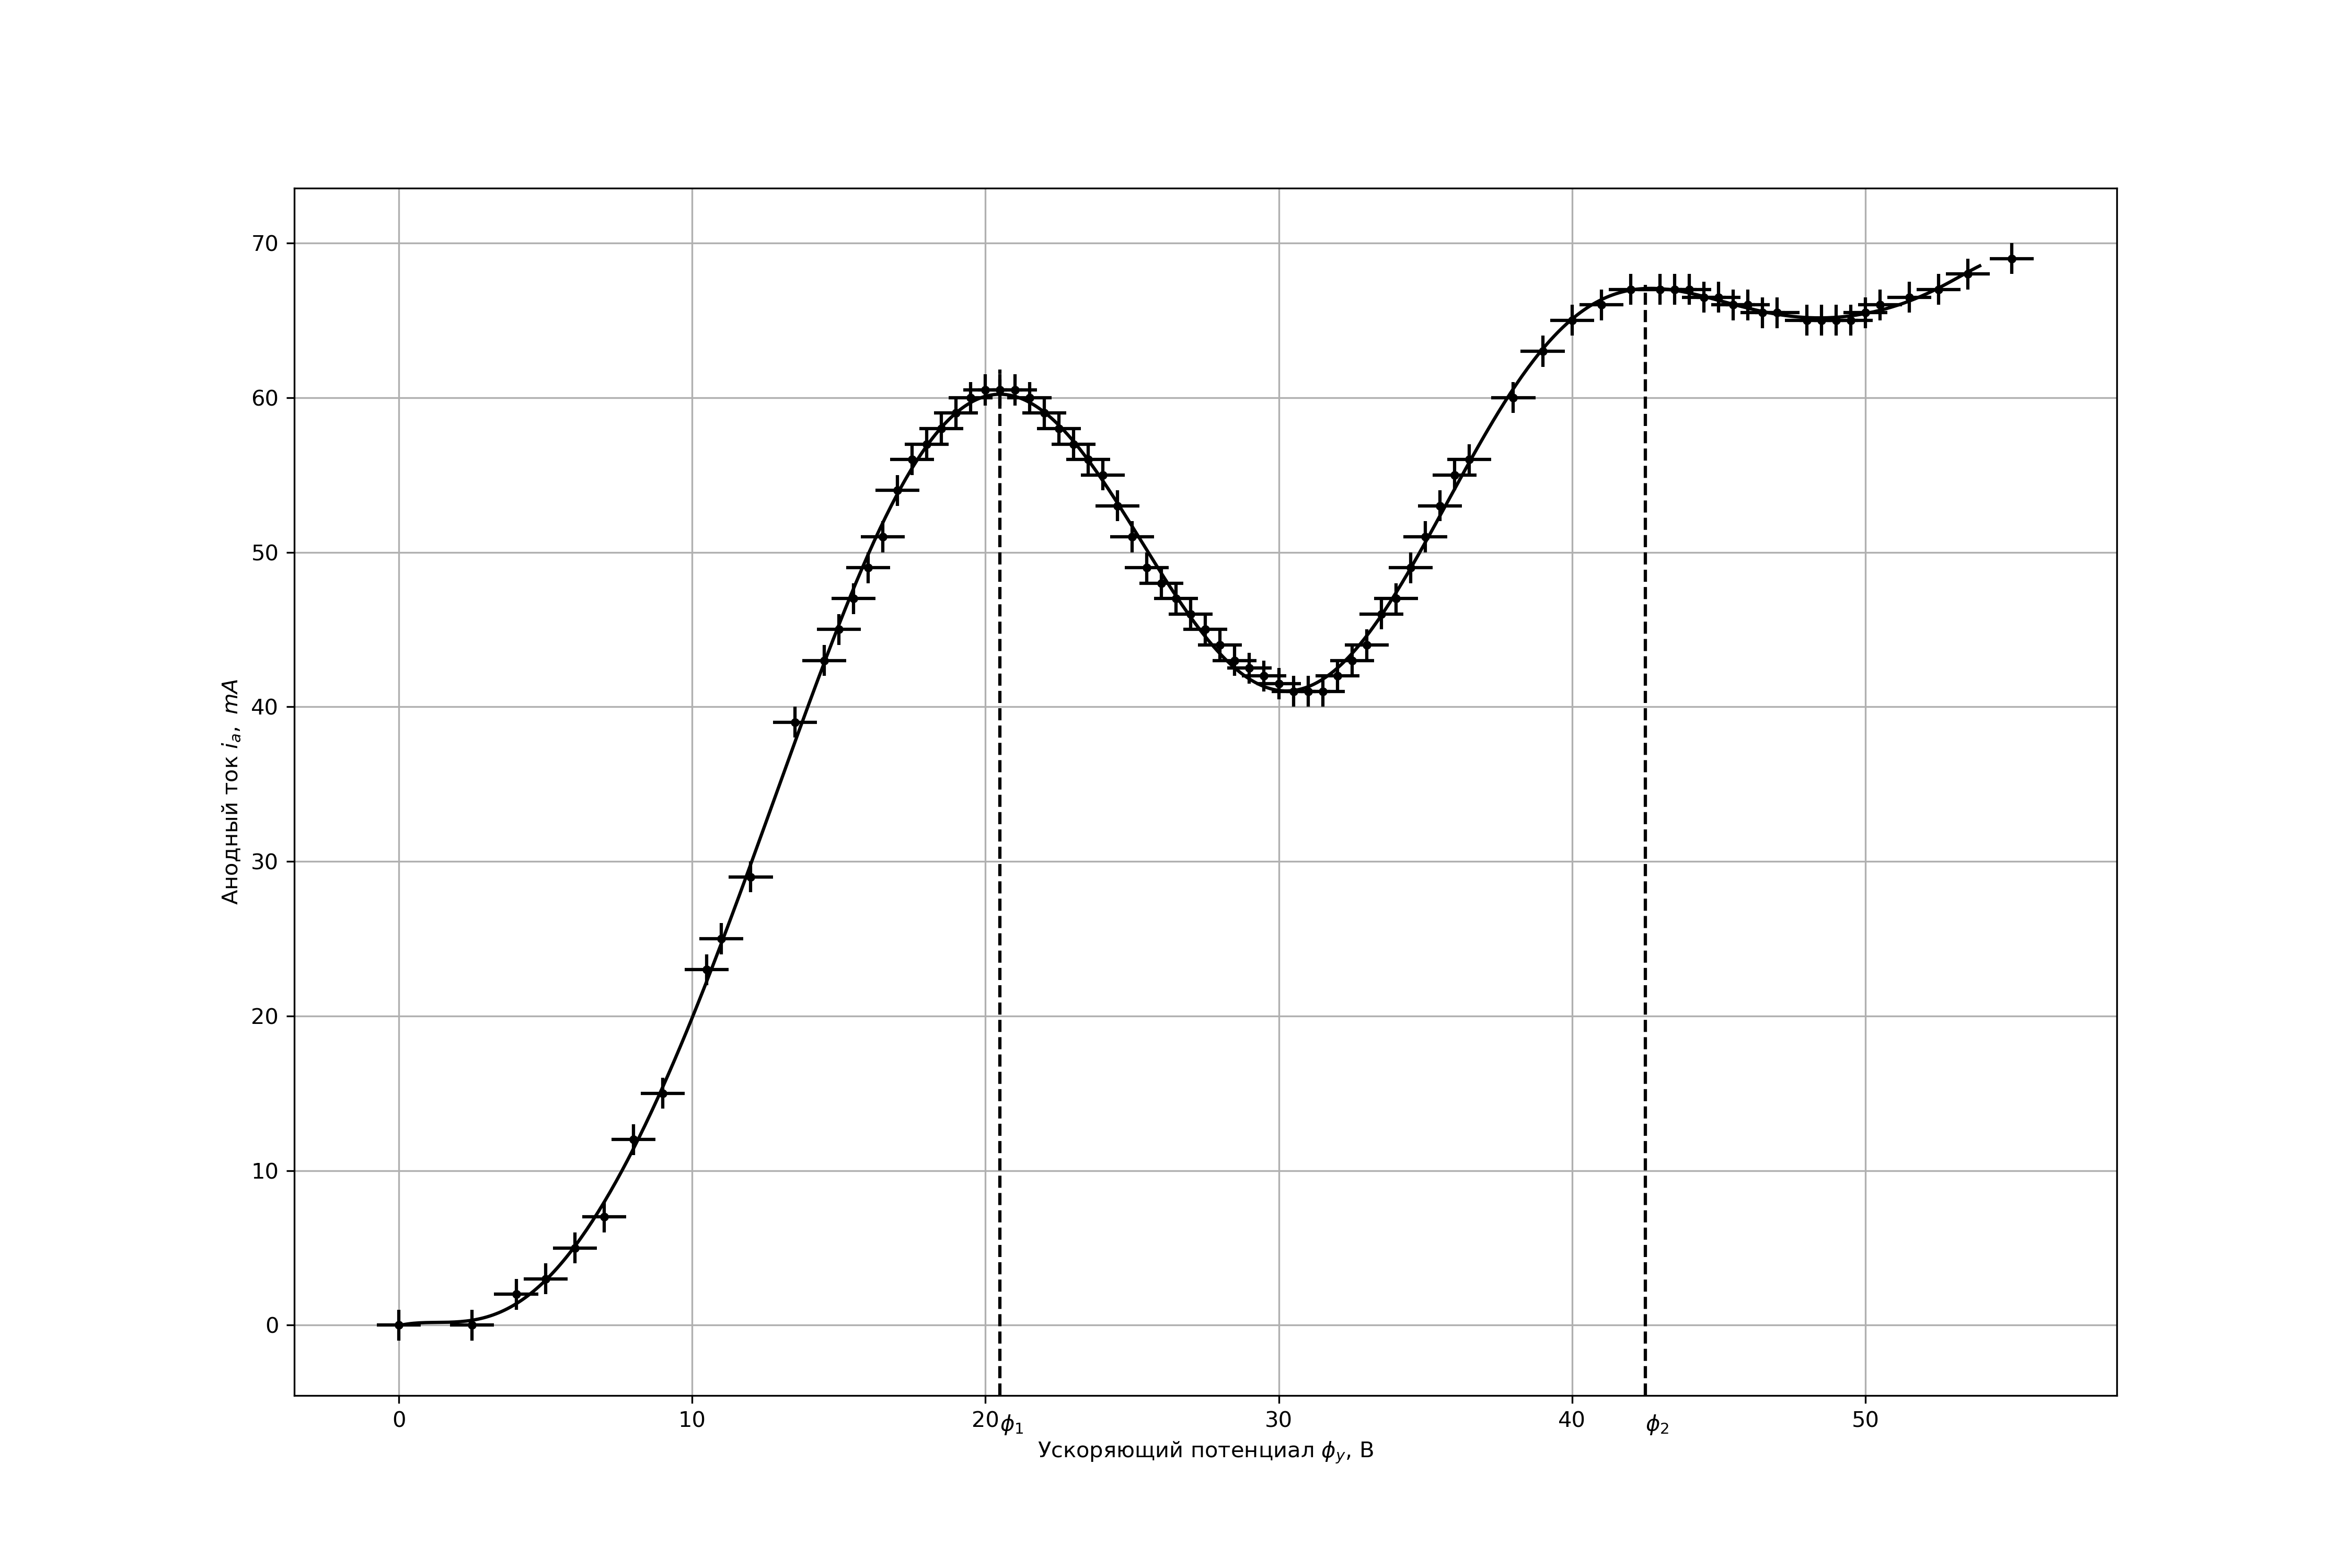
\includegraphics[width=\linewidth]{1.jpg} 
%         \label{fig:2}
%         \vspace{-32pt}
%         \captionof{figure}{} 
%     \end{minipage}
% \end{center}



\newpage
\section{Экспериментальная часть}



\end{document}